\documentclass[11pt,a4paper]{scrartcl}

% Pakete
\usepackage[english]{babel}
\usepackage[UKenglish]{isodate}
\usepackage{xcolor}
\usepackage{graphicx}
\usepackage{amsmath}
\usepackage{amssymb}
\usepackage{nicefrac}
\usepackage[utf8]{inputenc}
\usepackage{siunitx}
\sisetup{
output-decimal-marker={.},
exponent-product=\cdot }
\usepackage{esvect}
\usepackage{eqnarray}
\usepackage{placeins}
\usepackage{scrpage2}
\usepackage{nameref}
\usepackage{upgreek}
\usepackage{caption}
\usepackage{subcaption}
\usepackage{bm}
\usepackage{mwe}
\usepackage{tcolorbox}
\usepackage{listings}
\usepackage{xstring}
\usepackage{stringstrings}
\usepackage{floatflt}
\usepackage{pgfplots}
\usepackage{tikz}
%\usepackage{physics}


% Custom colors
\definecolor{deepblue}{rgb}{0,0,0.5}
\definecolor{deepred}{rgb}{0.6,0,0}
\definecolor{deepgreen}{rgb}{0,0.5,0}
\DeclareFixedFont{\ttb}{T1}{txtt}{bx}{n}{12} % for bold
\DeclareFixedFont{\ttm}{T1}{txtt}{m}{n}{12}  % for normal

% tikz
\usetikzlibrary{arrows}

% caption setup
\captionsetup[subfigure]{labelformat=simple, labelsep=colon}
\renewcaptionname{english}{\figurename}{Fig.}
\renewcommand{\thesubfigure}{\arabic{figure}.\arabic{subfigure}}
\renewcommand{\thesubtable}{\arabic{table}.\arabic{subtable}}

% Listning Einstellungen
\lstloadlanguages{python}       % Default highlighting set to "python"
\DeclareCaptionFont{white}{\color{white}}
\DeclareCaptionFormat{listing}{%
  \parbox{0.99\textwidth}{\colorbox{gray}{\parbox{0.99\textwidth}{#1#2#3}}\vskip+5pt}}
\captionsetup[lstlisting]{format=listing, labelfont=white, textfont=white}
\lstset{frame=lrb,xleftmargin=\fboxsep,xrightmargin=-\fboxsep}
\pagestyle{empty}
\lstset{escapeinside={<@}{@>}}
\lstdefinestyle{MyPythonStyle}{
		language=Python,
		numbers=left,
		breaklines=true,
		basicstyle=\ttm,
		otherkeywords={self},             % Add keywords here
		keywordstyle=\ttb\color{deepblue},
		emph={MyClass,__init__},          % Custom highlighting
		emphstyle=\ttb\color{deepred},    % Custom highlighting style
		stringstyle=\color{deepgreen},
		frame=tb,                         % Any extra options here
		showstringspaces=false            % 
		}
\lstdefinestyle{MyCStyle}{
		language=C,
		numbers=left,
		tabsize=4,
		breaklines=true,
		basicstyle=\ttm,
		otherkeywords={self},             % Add keywords here
		keywordstyle=\ttb\color{deepblue},
		emph={MyClass,__init__},          % Custom highlighting
		emphstyle=\ttb\color{deepred},    % Custom highlighting style
		stringstyle=\color{deepgreen},
		frame=tb,                         % Any extra options here
		showstringspaces=false            % 
		}
\renewcommand{\lstlistingname}{Code block}
\renewcommand{\lstlistlistingname}{List of \lstlistingname s}

% Griechische Buchstaben vereinheitlichen
\renewcommand{\alpha}{\upalpha}
\renewcommand{\beta}{\upbeta}
\renewcommand{\gamma}{\upgamma}
\renewcommand{\delta}{\updelta}
\newcommand{\w}{\omega}
\newcommand{\la}{\lambda}

% Eigene mathematische Kommandos
\newcommand{\dd}{\text{d}} 							% Differential
\newcommand{\p}{\partial} 								% Partielles Differential
\newcommand{\D}{\Delta} 								% Fehler / Laplace
\newcommand{\order}[1]{\mathcal{O}\left( #1 \right)}
\newcommand{\abs}[1]{\left| #1\right|} 					% Betrag
\newcommand{\Max}[1]{\max \left\lbrace #1\right\rbrace} % max{}
\newcommand{\Min}[1]{\min \left\lbrace #1\right\rbrace} % min{}
\newcommand{\diff}[2]{\frac{\text{d} #1}{\text{d} #2}}	% Ableitung
\newcommand{\pdiff}[2]{\frac{\partial #1}{\partial #2}} % Partielle Ableitung
\newcommand{\errprop}[2]{\left| \frac{\partial #1}{\partial #2}\right| \cdot \Delta #2}
														% Fehlerfortpflanzung
\newcommand{\rel}[1]{\frac{\Delta #1}{#1}}				% Relativer Fehler

% Eigene trigonometrische Funktionen
\newcommand{\Exp}[1]{\text{exp}\left( #1 \right)}		% exp()
\newcommand{\Ln}[1]{\text{ln}\left( #1 \right)}			% ln()
\newcommand{\Log}[1]{\text{log}\left( #1 \right)}		% log()
\newcommand{\Sin}[1]{\text{sin}\left( #1 \right)}     	% sin()
\newcommand{\Cos}[1]{\text{cos}\left( #1 \right)}		% cos()
\newcommand{\Sinz}[1]{\text{sin}^2\left( #1 \right)}	% sin^2()
\newcommand{\Cosz}[1]{\text{cos}^2\left( #1 \right)}	% cos^2()
\newcommand{\Tan}[1]{\text{tan}\left( #1 \right)}		% tan()
\newcommand{\Asin}[1]{\text{asin}\left( #1 \right)}		% asin()
\newcommand{\Acos}[1]{\text{acos}\left( #1 \right)}		% acos()
\newcommand{\Atan}[1]{\text{atan} \left( #1 \right)}	% atan()

% Eigene Vektor Kommandos
\newcommand{\tovec}[2]{\begin{pmatrix}#1\\ #2\end{pmatrix}}	% 2D-Vektor
\newcommand{\trvec}[3]{\begin{pmatrix}#1\\ #2\\ #3\end{pmatrix}}	% 3D-Vektor	
\newcommand{\ovec}[1]{\boldsymbol{#1}}

% Eigene Referenz-Kommandos
\newcommand{\eref}[1]{(\ref{#1})}						% Gleichungen
\newcommand{\sref}[2]{\subref{#2}}						% Unterabbildungen
\newcommand{\kref}[1]{\ref{#1} \glqq\nameref{#1}\grqq}  % Kapitel
\newcommand{\lref}[1]{$[#1]$}							% Quellen: \newcommand{\lit}{1} => \lref{\lit}

% listing commandos
\newcommand{\listfile}[7][MyPythonStyle]{
\lstinputlisting[linerange={#4-#5}, firstnumber=#4, caption={#6} \hfill script:  #3, label=#7, style=#1]{#2}}
% arguments:
% \listfile[style]{location/filename}{filename}{firstline}{lastline}{title}{label}
% Imports code from a file 
% You will have to escape the filename and the title
% style is an optional argument.

\newcommand{\ls}[1]{\lstinline@#1@}

% using \lstinline@code@ for code in line
% works with every sign instead of @

% commands for this task
\newcommand{\ua}{AU}
\newcommand{\vecx}[1]{\ovec{x}^{(#1)}}
\newcommand{\vecv}[1]{\ovec{v}^{(#1)}}
\newcommand{\veca}[1]{\ovec{a}^{(#1)}}
\newcommand{\vecF}[1]{\ovec{F}^{(#1)}}
\newcommand{\vecr}[1]{\ovec{r}^{(#1)}}
\newcommand{\nx}[1]{x^{(#1)}}
\newcommand{\nv}[1]{v^{(#1)}}
\newcommand{\na}[1]{a^{(#1)}}
\newcommand{\nm}[1]{m^{(#1)}}
\newcommand{\nF}[1]{F^{(#1)}}
\newcommand{\nr}[1]{r^{(#1)}}
\newcommand{\Ekin}{E_\text{kin}}
\newcommand{\Ekino}{E_{\text{kin},0}}
\newcommand{\fr}{f_\text{re}}
\newcommand{\fij}{\ovec{f}_{ij}}
\newcommand{\rij}{\ovec{r}_{ij}}
\newcommand{\fji}{\ovec{f}_{ji}}
\newcommand{\rji}{\ovec{r}_{ji}}
\newcommand{\rj}{\ovec{r}_{j}}
\newcommand{\ri}{\ovec{r}_{i}}



% Kopf-/Fusszeile
\pagestyle{scrheadings}
\clearscrheadfoot
\chead{Simulation Methods in Physics I}
\ihead{Worksheet 3}
\ohead{\today}
\ofoot{\pagemark}
\ifoot{Michael Marquardt, Cameron Stewart}

\begin{document}

% Titelseite
\begin{titlepage}

\ \\ \ \\ \ \\

\center\textbf{
\begin{large}
Simulation Methods in Physics I
\end{large} \\ \ \\
\begin{Large}
Worksheet 4: Thermostats
\end{Large}}   \\ \ \\
\ \\ \ \\

\begin{tabular}{lll}
Students: &Michael Marquardt &Cameron Stewart\\ 
matriculation numbers: &3122118 &3216338\\
\end{tabular}

\end{titlepage}

% Inhaltsverzeichnis

% -------------------------------------- Begin Of Document ----------------------------------------

\section{Random Numbers}

All the functions for this task are implemented in random\_numbers.py.
The file random\_walk.py executes the code.

\subsection{Linear Congruental Gemerator (LCG)}

The first exercise was to implement the LCG.
In order to do this the LCG must be initialized with an overall value Xlcg.

\listfile{../src/random_numbers.py}{src/random\_numbers.py}{5}{9}{Initialization of LCG}{initlcg}

The next step is to perform the LCG; therefore a function LCG() is implemented in code block \ref{lcg}.
As you can see the values m, a and c are already given as optional parameters.

\listfile{../src/random_numbers.py}{src/random\_numbers.py}{11}{17}{LCG}{lcg}

Later we want to use the time.time() as a starting value. 
Therefore the function do2int() is defined which converts a float into an integer by passing the decimal marker after the last relevant number.

\listfile{../src/random_numbers.py}{src/random\_numbers.py}{25}{32}{do2int}{do2int}

At last the function normal\_LCG() returns a normalized value in [0,1].
Therefore the result must be divided by m-1.\\

Now it is time to run the random number generator and simulate a random walk. 
Therefor the function random\_walk() is used to generate an 1D random walk with a maximum velocity of $\pm 0.5$ per time step.

\listfile{../src/random_numbers.py}{src/random\_numbers.py}{34}{47}{Random walk}{walk}

The script random\_walk.py takes an optional command line parameter --Xlcg. 
You can use it to set the starting value Xlcg manually.
If it is not given do2int(time.time()) is used.
Notice, that you have to use python3 in order to get good results from the time function.\\

If you perform the random walk several times with the same --Xlcg the trajectory appears to be the same every time. 
By using time.time() as initialization you obey completely different trajectories every time. 
You can see one of this trajectories in graphic \ref{randwalk}.

\begin{figure}[ht]
	\centering
	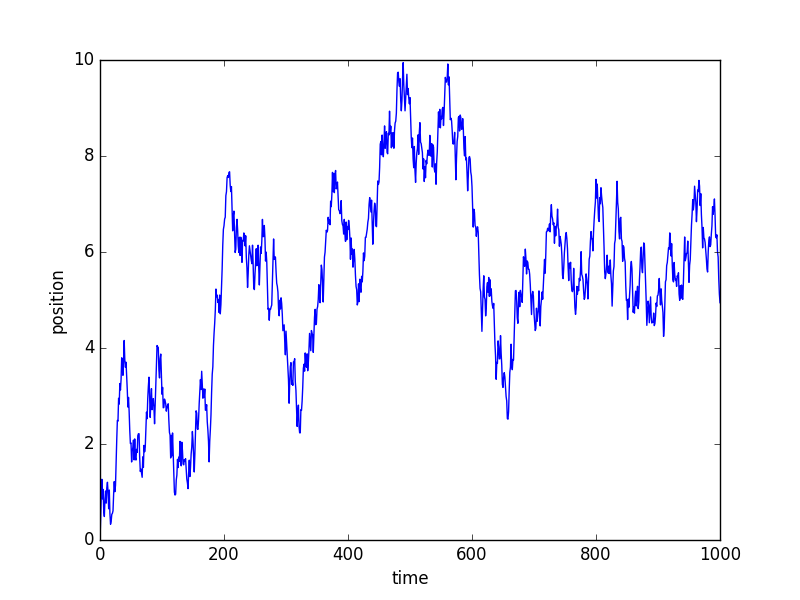
\includegraphics[width=0.7\textwidth]{../dat/random_walk.png}
	\caption{
		Random walk for initialization with time.time().
		}
	\label{randwalk}
\end{figure}

To conclude, the LCG is not really a good random number generator.
Although it takes a long time until the numbers repeat in the same order in between, there can be no number which was already obeyed.
Due to this the random numbers are correlated especially for many used numbers.
Furthermore a bad choice of m, a and c will lead to very bad and no longer uniform random number distribution.

\FloatBarrier

\subsection{Box-Muller (BM)}

The next exercise is to transform uniformly distributed random numbers into 
normal distributed one. 
Therefor the Box-Muller transform is given.
It's implementation is split up into two functions.
calc\_BM() takes two uniform distributed random numbers u1 and u2 and returns the function from the worksheet. 
The function BM() arranges the usage of calc\_BM() in a way that allows to obey an array of $N>1$ normal distributed random numbers. 
In order to get better results the function random.random() which returns better uniformly distributed random numbers is used instead of LCG().

\listfile{../src/random_numbers.py}{src/random\_numbers.py}{51}{65}{Box-Muller}{bm}

The function gauss() just returns the Gaussian probability distribution:
\begin{align}
p(x) 
	&= \frac{1}{\sqrt{2\pi}\sigma}\dot{\Exp{-\frac{x^2}{2\sigma^2}}}
	\label{gauss}
\end{align}

Analogous the function gauss\_3d() returns the three dimensional Gaussian:
\begin{align}
p(\ovec{r}) 
&= \sqrt{\frac{2}{\pi}}\frac{\ovec{r}^2}{\sigma^3}\dot{\Exp{-\frac{\ovec{r}^2}{2\sigma^2}}}
\label{gauss3d}
\end{align}

In order to test the BM a function show\_BM\_hist() was created.
It draws a histogram of 1000 by the BM() created random numbers in a diagram with the gauss().
You can pass different $\sigma$, $\mu$ and therefor also new x-axis-limits.
The option bars states how many bars you want to have for the histogram.
The results can be seen in graphic \ref{bmhist}.

\listfile{../src/random_numbers.py}{src/random\_numbers.py}{73}{88}{Box-Muller histogram}{showbmhist}

\begin{figure}[ht]
	\centering
	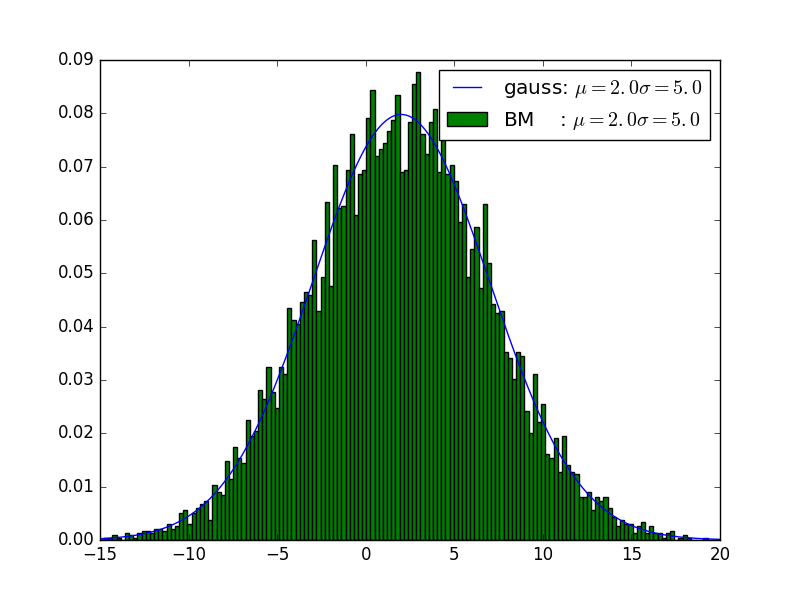
\includegraphics[width=0.7\textwidth]{../dat/BM_hist.png}
	\caption{
		Histogram of the BM random number distribution and the Gaussian function \eqref{gauss}.
	}
	\label{bmhist}
\end{figure}

The last exercise was to transform the same principal into three dimensions.
You can use the function rand\_vel\_vec() in order to create a $N\times 3$ vector of BM random numbers (velocity vector). 
The function show\_vel\_hist() in code block \ref{showvelhist} takes the absolute values of this velocities vel\_abs and draws them as histogram against the three dimensional Gaussian \eqref{gauss3d}.

\listfile{../src/random_numbers.py}{src/random\_numbers.py}{105}{120}{3D Box-Muller histogram}{showvelhist}

\begin{figure}[ht]
	\centering
	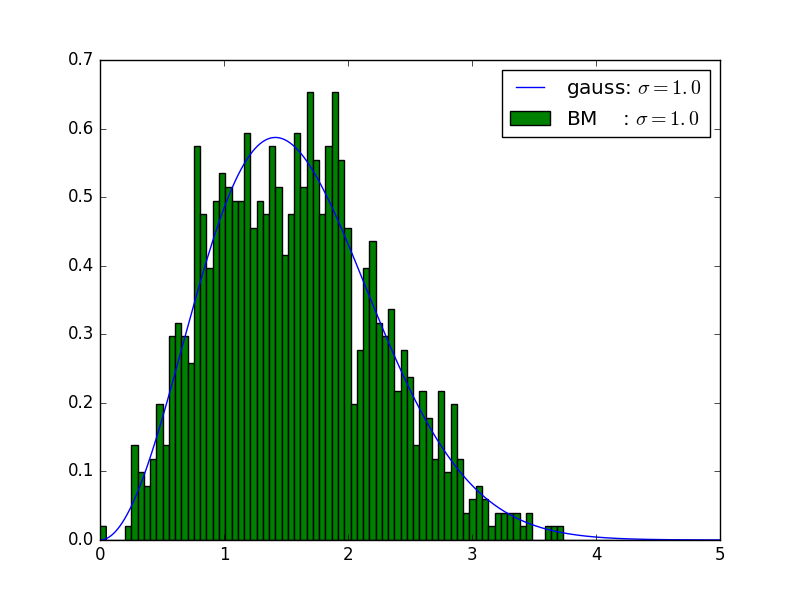
\includegraphics[width=0.7\textwidth]{../dat/vel_hist.png}
	\caption{
		Histogram of the BM random velocities and the 3D Gaussian function \eqref{gauss3d}.
	}
	\label{velhist}
\end{figure}

As you can see the histograms fit to the expected distribution in both cases.\\

Notice that it would not make sense to set an $\mu\neq 0$ unless you have a drift which means an overall velocity trend in a specific direction. 

\FloatBarrier
\section{Langevin Thermostat}

At first notice that the script ljsim.py was changed in such a way that you can pass more command line parameters via argparse.
The simulation ID is now passes via --ID.\\

The Langevin thermostat simulates a solvent in which causes friction and random forces (through collisions).
It allows to conserve the canonical (N,V,T)-ensemble.\\

\subsection{Implementation}

The implementation of the formulas which were given on the worksheet is done in code block \ref{langevin}.

\listfile{../src/ljsim.py}{src/ljsim.py}{94}{113}{Langevin thermostat}{langevin}

The random force is generated in line 114 with the the function $\ovec{W}_i(t)=\sqrt{12}\sigma\cdot a$ where a is a uniform random number between $-0.5$ and $0.5$ and the standard deviation $\sigma =\sqrt{\frac{2mk_BT\gamma}{\D t}}$.\\

The script allows to take the optional command line argument --gamma which is default $\gamma =0.3$.
Furthermore the main loop is modified in such a way, that it stores the trajectory, the velocities and the temperatures in the *.dat-file, so that you can not only restart the simulation but also get knowledge about the former simulation data.
The new command line parameter --restart allows you to restart a simulation instead of continuing it.

\subsection{Simulation}

Now the simulation can be performed. 
The desired temperature T\_des can be set by --T and is default 1.0.
The result of the simulation is shown as a plot of temperature over time \ref{langevinT}.

\begin{figure}[ht]
	\centering
	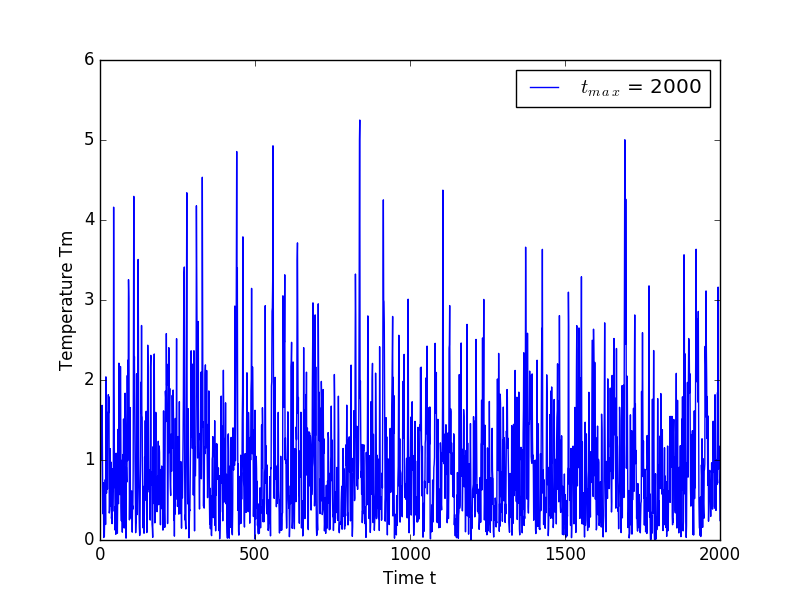
\includegraphics[width=0.7\textwidth]{../dat/langevin_T1d0_gamma0d3_Tm.png}
	\caption{
		Plot of the temperature over time for a desired temperature of $T_\text{des}=1.0$ for a simulation with the Langevin thermostat and $\gamma =0.3$.
	}
	\label{langevinT}
\end{figure}

In order to check weather the Maxwell-Boltzmann distribution for the velocities is fulfilled a histogram of the velocity distribution is drawn in figure \ref{langevinvv}.
Of course the distribution is meant over over time, because we are simulationg only one particle, but the script allows also to get a distribution also over all particles if we set other initial conditions with more than one particle.
For a physical system with Temperature $T$, the deviation is $\sigma =\sqrt{T}$.

\listfile{../src/ljsim.py}{src/ljsim.py}{290}{299}{Calculation of the histogram}{vvhist}

\begin{figure}[ht]
	\centering
	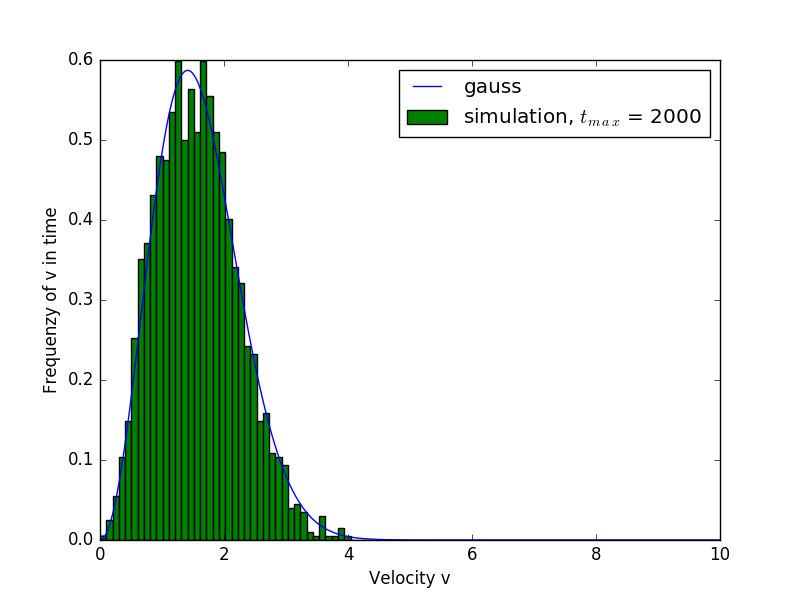
\includegraphics[width=0.7\textwidth]{../dat/langevin_T1d0_gamma0d3_vv.png}
	\caption{
		Histogram for the distribution of the absolute of the velocities in time for a desired temperature of $T_\text{des}=1.0$ for a simulation with the Langevin thermostat and $\gamma =0.3$.
	}
	\label{langevinvv}
\end{figure}

The figures show that the simulated velocity behaves like we physically expect it to behave. 
The temperature is varies around 1.0 with many high peaks in between, but the velocity distribution clearly fits the expected Gaussian.

\FloatBarrier
\section{Andersen Thermostat}

The Andersen thermostat is an easier model than the Langevin thermostat. 
As before we assume a solvent but now there is no friction but only random velocity replacement. 
We simply state, that a particle gets a normal distributed velocity through collisions with the solvent with a certain probability. 
The mean difference is that we are are not assuming a random \textbf{force} but a new random \textbf{velocity}, no matter which velocity the particle had before.
This is not physical!\\

Due to this the Andersen thermostat creates a (N,V,T)-ensemble, but not allows to determine dynamical properties of the system, because the random velocity replacement destroys the memory of the system (especially if there is only one particle or no interaction between particles).

\subsection{Implementation}

For the Andersen thermostat most parts of the existing script can be used.
The new part is the function step\_vv\_andersen() which you can see in code block \ref{andersen}.

\listfile{../src/ljsim.py}{src/ljsim.py}{115}{138}{Andersen thermostat}{andersen}

The function equals the original step\_vv() function except that there is the velocity replacement at the end.
In line 141 it loops over all particles.
This may not be necessary when simulating only one particle, but it allows to use other initial conditions for the same script with more than one particle.
The next line asks weather a random number is smaller than $\nu \D t$ where --nu allows you to pass a parameter nu (default: $\nu =0.1$).
This term represents the probability for a stochastic collision.
If the statement is fulfilled the velocity of the selected particle is replaced by a normal distributed random velocity with a deviation of $\sigma =\sqrt{T_\text{des}}$.

\subsection{Simulation}

Simulating with the Andersen thermostat works exactly like in the former task.
The results can be seen in the figures \ref{andersenT} and \ref{andersenvv}.

\begin{figure}[ht]
	\centering
	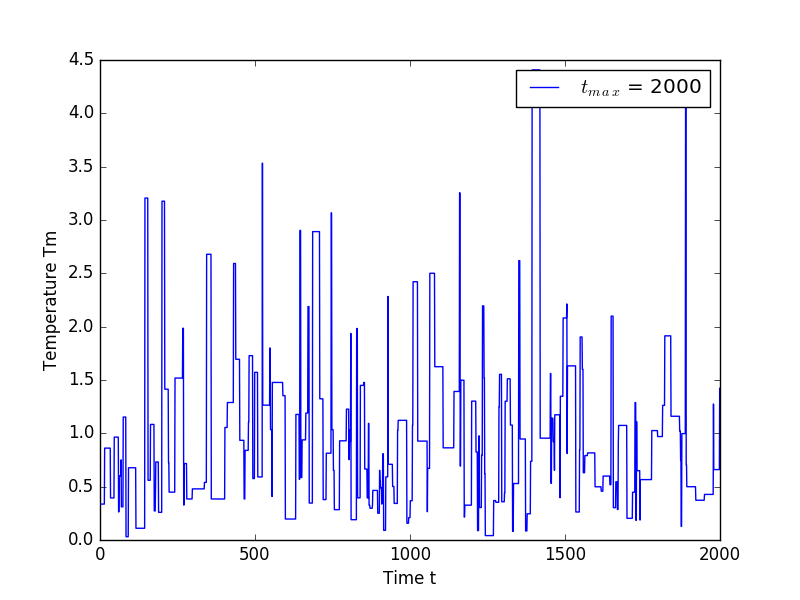
\includegraphics[width=0.7\textwidth]{../dat/andersen_T1d0_nu0d1_Tm.png}
	\caption{
		Plot of the temperature over time for a desired temperature of $T_\text{des}=1.0$ for a simulation with the Andersen thermostat and $\nu =0.3$.
	}
	\label{andersenT}
\end{figure}

\begin{figure}[ht]
	\centering
	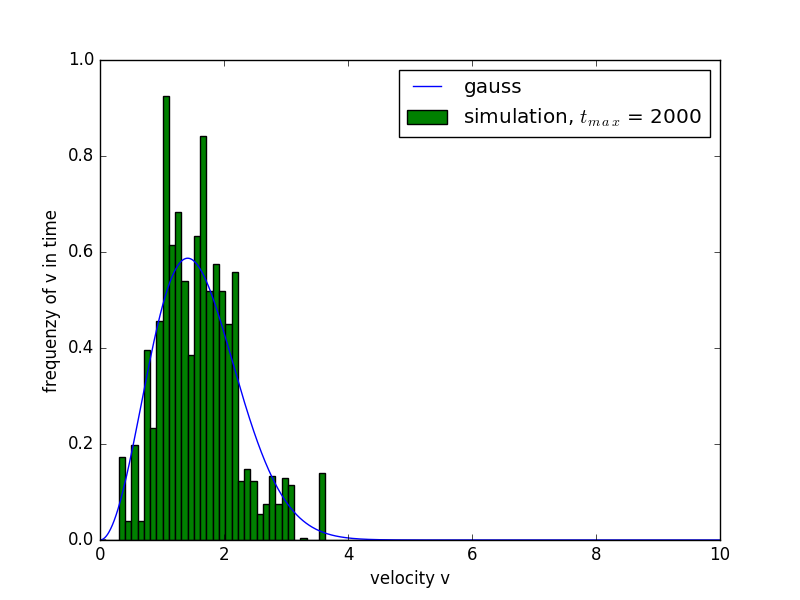
\includegraphics[width=0.7\textwidth]{../dat/andersen_T1d0_nu0d1_vv.png}
	\caption{
		Plot of the temperature over time for a desired temperature of $T_\text{des}=1.0$ for a simulation with the Andersen thermostat and $\nu =0.3$.
	}
	\label{andersenvv}
\end{figure}

As you can see the temperature is also varying around 1.0 but not with the same regularity. 
The velocity distribution comes near to the Gaussian but it does not fit as good as for the Langevin thermostat.

\FloatBarrier 

\section{Berendsen Thermostat}

The Berendsen thermostat is very similar to the velocity-rescaling on the former worksheet.
It just multiplies the velocities of all particles with a factor $\lambda =\sqrt{1+\frac{\D t}{\tau_T}\left(\frac{T_\text{des}}{T_\text{act}}-1\right) }$ so that the 
Thereby $T_\text{act}$ is the actual temperature. 
As the mentioned velocity-rescaling this thermostat does no physical stuff and is not useful for observing the dynamics of a system.

\subsection{Implementation}

The implementation is as easy as possible.
The function step\_vv\_berendsen() equals step\_vv() but in line 159 the temperature is measured in order to rescale velocities in line 160.

\listfile{../src/ljsim.py}{src/ljsim.py}{140}{162}{Berendsen thermostat}{berendsen}

The parameter tau ($\tau_T$) can be set by --tau and has a default value of 3.0.

\subsection{Simulation}

The simulation is done in the same way as for the other thermostats. 
The results can be seen in the figures \ref{berendsenT} and \ref{berendsenvv}.

\begin{figure}[ht]
	\centering
	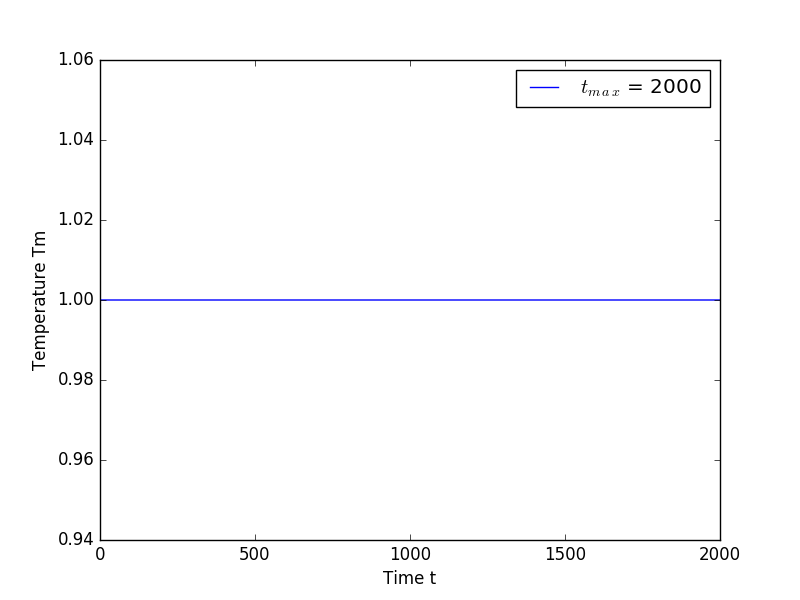
\includegraphics[width=0.7\textwidth]{../dat/berendsen_T1d0_tau3d0_Tm.png}
	\caption{
		Plot of the temperature over time for a desired temperature of $T_\text{des}=1.0$ for a simulation with the Andersen thermostat and $\tau_T =3.0$.
	}
	\label{berendsenT}
\end{figure}

\begin{figure}[ht]
	\centering
	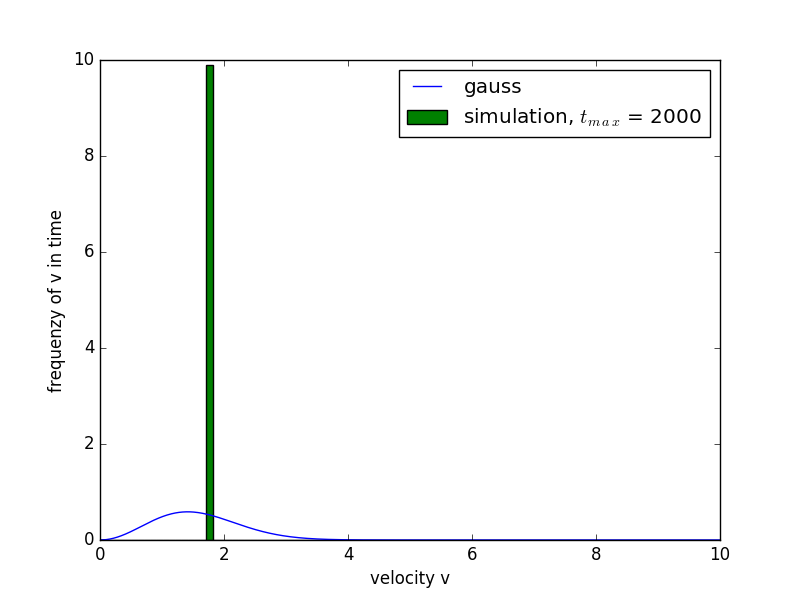
\includegraphics[width=0.7\textwidth]{../dat/berendsen_T1d0_tau3d0_vv.png}
	\caption{
		Plot of the temperature over time for a desired temperature of $T_\text{des}=1.0$ for a simulation with the Berendsen thermostat and $\tau_T =3.0$.
	}
	\label{berendsenvv}
\end{figure}

As you can see the results differ from the further tasks.
The temperature is constant at the desired temperature 1.0. 
There is no fluctuation any more.
It is the same for the velocities. 
The velocity stays constant at a value which gives us the right temperature. 
There is no Gaussian at all.
Of course this will look different for more than one particle with pair interactions, but it would also not fulfill the Gaussian.\\

Because of this the Berendsen thermostat is the worst of the three thermostats (in a physical meaning).

\FloatBarrier
\section{Diffusion}




\end{document}
